\documentclass{standalone}
\usepackage{tikz}
\usetikzlibrary{patterns, positioning}
\usepackage[sfdefault]{ClearSans} %% option 'sfdefault' activates Clear Sans as the default text font
\usepackage[T1]{fontenc}

\begin{document}
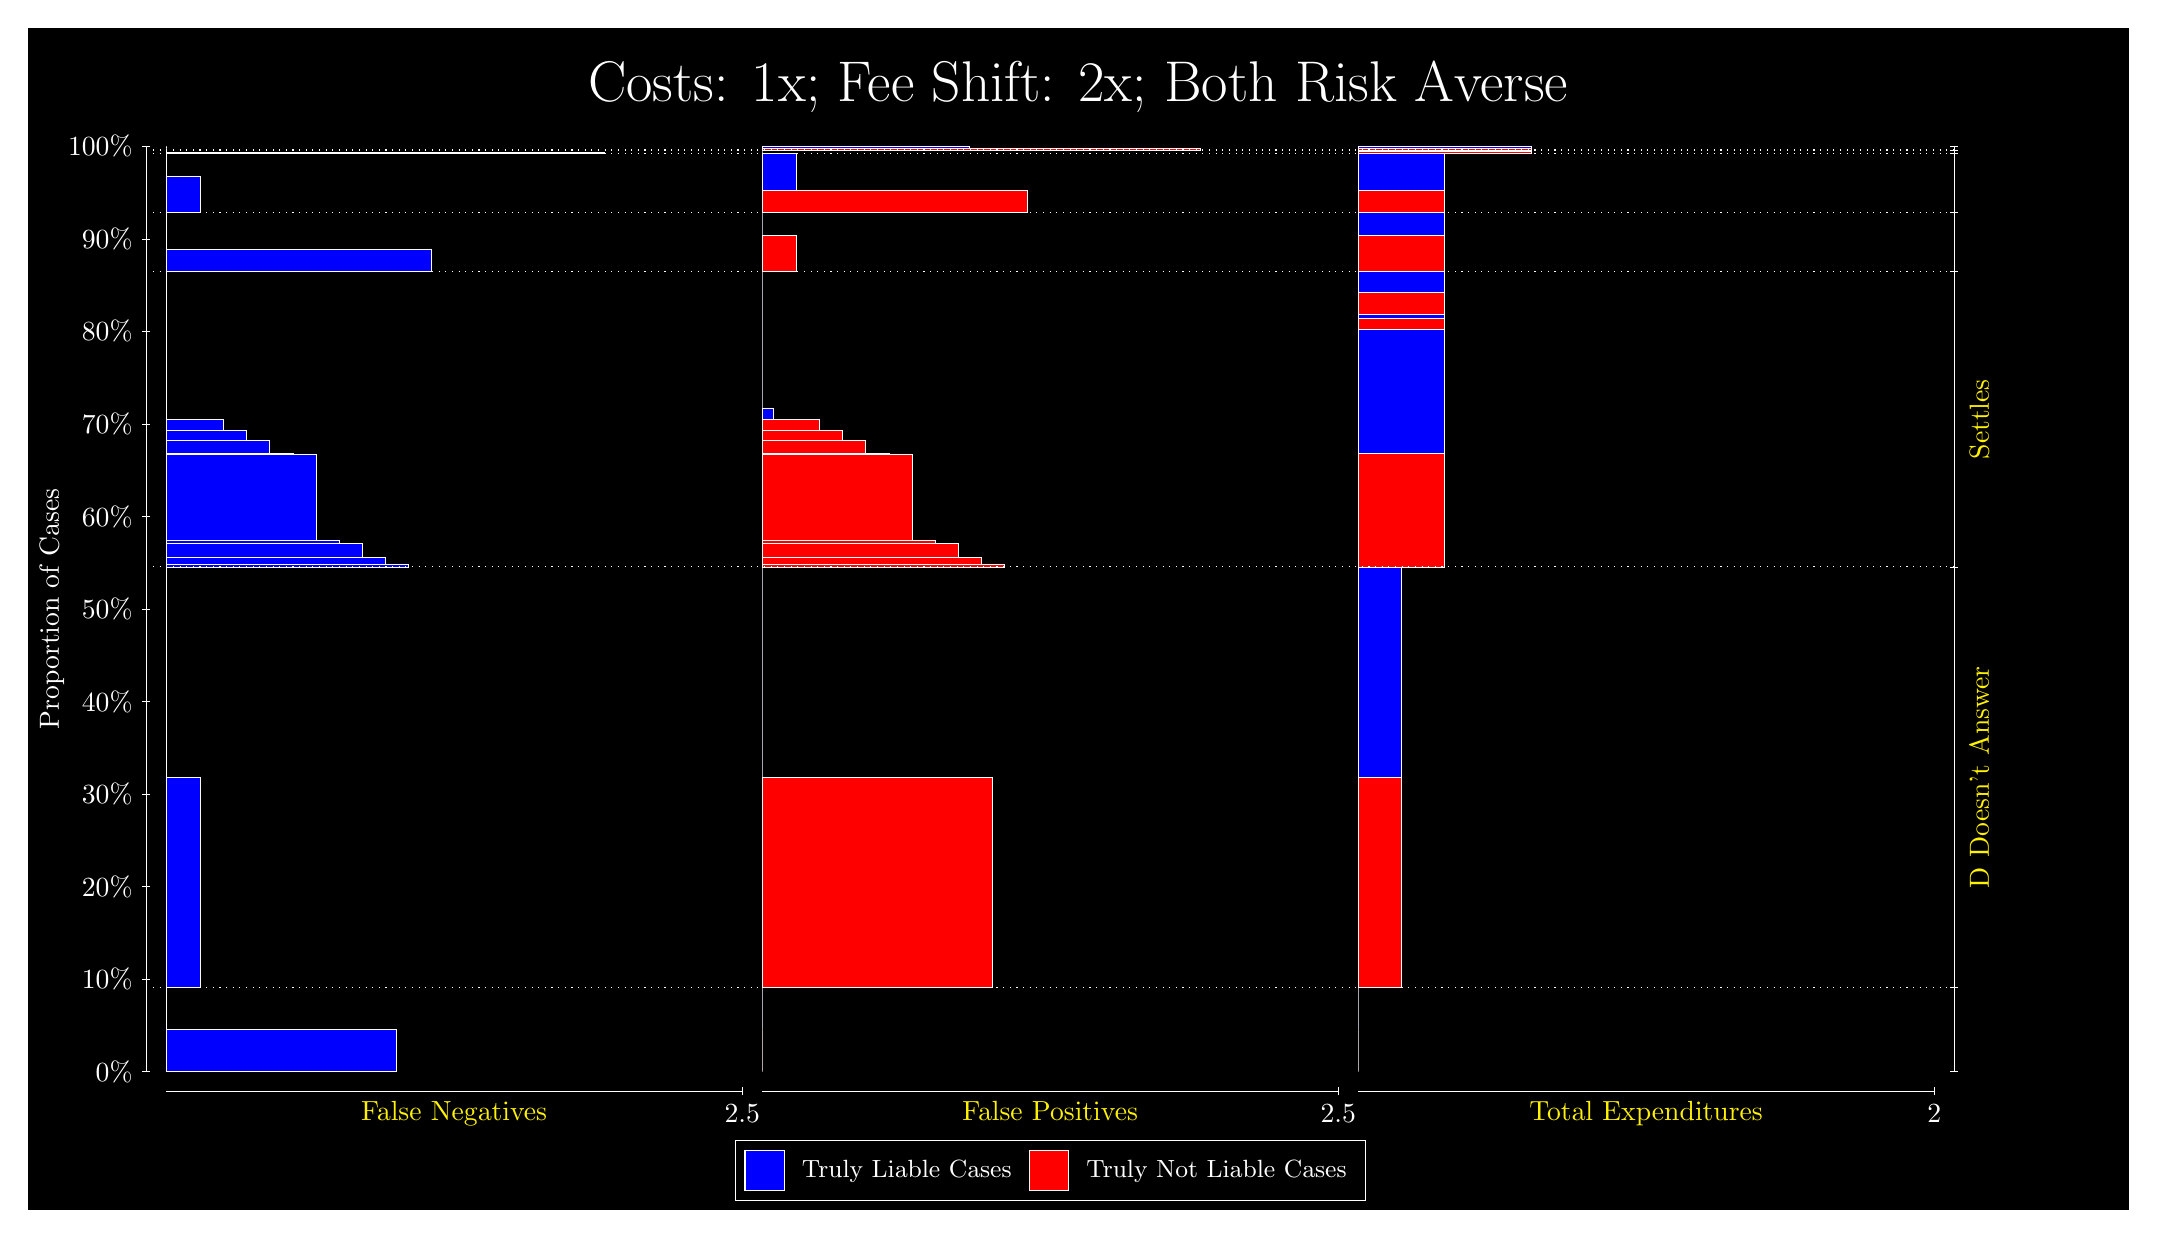
\begin{tikzpicture}
\draw[fill=black] (0,0) rectangle (26.667,15);
\draw[text=white] (0,13.5) rectangle (26.667,15) node[midway] {\huge Costs: 1x; Fee Shift: 2x; Both Risk Averse};
\draw[white, very thin] (1.5,1.75) -- (1.5,13.5);
\node[rotate=90, text=white, anchor=center] at (0.3, 7.625) {Proportion of Cases};
\draw[white, very thin] (1.45,1.75) -- (1.55,1.75);
\node[text=white, anchor=east] at (1.45, 1.75) {0\%};
\draw[white, very thin] (1.45,2.925) -- (1.55,2.925);
\node[text=white, anchor=east] at (1.45, 2.925) {10\%};
\draw[white, very thin] (1.45,4.1) -- (1.55,4.1);
\node[text=white, anchor=east] at (1.45, 4.1) {20\%};
\draw[white, very thin] (1.45,5.275) -- (1.55,5.275);
\node[text=white, anchor=east] at (1.45, 5.275) {30\%};
\draw[white, very thin] (1.45,6.45) -- (1.55,6.45);
\node[text=white, anchor=east] at (1.45, 6.45) {40\%};
\draw[white, very thin] (1.45,7.625) -- (1.55,7.625);
\node[text=white, anchor=east] at (1.45, 7.625) {50\%};
\draw[white, very thin] (1.45,8.8) -- (1.55,8.8);
\node[text=white, anchor=east] at (1.45, 8.8) {60\%};
\draw[white, very thin] (1.45,9.975) -- (1.55,9.975);
\node[text=white, anchor=east] at (1.45, 9.975) {70\%};
\draw[white, very thin] (1.45,11.15) -- (1.55,11.15);
\node[text=white, anchor=east] at (1.45, 11.15) {80\%};
\draw[white, very thin] (1.45,12.325) -- (1.55,12.325);
\node[text=white, anchor=east] at (1.45, 12.325) {90\%};
\draw[white, very thin] (1.45,13.5) -- (1.55,13.5);
\node[text=white, anchor=east] at (1.45, 13.5) {100\%};

\draw[white, very thin] (24.457,1.75) -- (24.457,13.5);
\draw[white, very thin] (24.407,1.75) -- (24.507,1.75);
\node[anchor=west] at (24.407, 1.75) {};
\draw[white, very thin] (24.407,2.8182) -- (24.507,2.8182);
\node[anchor=west] at (24.407, 2.8182) {};
\draw[white, very thin] (24.407,8.1591) -- (24.507,8.1591);
\node[anchor=west] at (24.407, 8.1591) {};
\draw[white, very thin] (24.407,11.91) -- (24.507,11.91);
\node[anchor=west] at (24.407, 11.91) {};
\draw[white, very thin] (24.407,12.658) -- (24.507,12.658);
\node[anchor=west] at (24.407, 12.658) {};
\draw[white, very thin] (24.407,13.406) -- (24.507,13.406);
\node[anchor=west] at (24.407, 13.406) {};
\draw[white, very thin] (24.407,13.453) -- (24.507,13.453);
\node[anchor=west] at (24.407, 13.453) {};
\draw[white, very thin] (24.407,13.5) -- (24.507,13.5);
\node[anchor=west] at (24.407, 13.5) {};

\draw[white, very thin, fill=blue] (1.75,1.75) rectangle (4.6775,2.2841);
\draw[white, very thin, fill=red] (1.75,2.2841) rectangle (1.75,2.8182);
\draw[white, very thin, fill=blue] (1.75,2.8182) rectangle (2.1891,5.4886);
\draw[white, very thin, fill=red] (1.75,5.4886) rectangle (1.75,8.1591);
\draw[white, very thin, fill=blue] (1.75,8.1591) rectangle (4.8239,8.1983);
\draw[white, very thin, fill=blue] (1.75,8.1983) rectangle (4.5312,8.2776);
\draw[white, very thin, fill=blue] (1.75,8.2776) rectangle (4.2384,8.4628);
\draw[white, very thin, fill=blue] (1.75,8.4628) rectangle (3.9457,8.4996);
\draw[white, very thin, fill=blue] (1.75,8.4996) rectangle (3.6529,9.5953);
\draw[white, very thin, fill=blue] (1.75,9.5953) rectangle (3.3602,9.6076);
\draw[white, very thin, fill=blue] (1.75,9.6076) rectangle (3.0674,9.7718);
\draw[white, very thin, fill=blue] (1.75,9.7718) rectangle (2.7746,9.8914);
\draw[white, very thin, fill=blue] (1.75,9.8914) rectangle (2.4819,10.034);
\draw[white, very thin, fill=red] (1.75,10.034) rectangle (1.75,11.91);
\draw[white, very thin, fill=blue] (1.75,11.91) rectangle (5.1167,12.197);
\draw[white, very thin, fill=red] (1.75,12.197) rectangle (1.75,12.658);
\draw[white, very thin, fill=blue] (1.75,12.658) rectangle (2.1891,13.119);
\draw[white, very thin, fill=red] (1.75,13.119) rectangle (1.75,13.406);
\draw[white, very thin, fill=blue] (1.75,13.406) rectangle (7.3123,13.423);
\draw[white, very thin, fill=red] (1.75,13.423) rectangle (1.75,13.453);
\draw[white, very thin, fill=red] (1.75,13.453) rectangle (1.75,13.471);
\draw[white, very thin, fill=blue] (1.75,13.471) rectangle (1.75,13.5);
\draw[white, very thin, fill=red] (9.3189,1.75) rectangle (9.3189,2.2841);
\draw[white, very thin, fill=blue] (9.3189,2.2841) rectangle (9.3189,2.8182);
\draw[white, very thin, fill=red] (9.3189,2.8182) rectangle (12.246,5.4886);
\draw[white, very thin, fill=blue] (9.3189,5.4886) rectangle (9.3189,8.1591);
\draw[white, very thin, fill=red] (9.3189,8.1591) rectangle (12.393,8.1983);
\draw[white, very thin, fill=red] (9.3189,8.1983) rectangle (12.1,8.2776);
\draw[white, very thin, fill=red] (9.3189,8.2776) rectangle (11.807,8.4628);
\draw[white, very thin, fill=red] (9.3189,8.4628) rectangle (11.515,8.4996);
\draw[white, very thin, fill=red] (9.3189,8.4996) rectangle (11.222,9.5953);
\draw[white, very thin, fill=red] (9.3189,9.5953) rectangle (10.929,9.6076);
\draw[white, very thin, fill=red] (9.3189,9.6076) rectangle (10.636,9.7718);
\draw[white, very thin, fill=red] (9.3189,9.7718) rectangle (10.344,9.8914);
\draw[white, very thin, fill=red] (9.3189,9.8914) rectangle (10.051,10.034);
\draw[white, very thin, fill=blue] (9.3189,10.034) rectangle (9.4652,10.177);
\draw[white, very thin, fill=blue] (9.3189,10.177) rectangle (9.3189,11.91);
\draw[white, very thin, fill=red] (9.3189,11.91) rectangle (9.758,12.371);
\draw[white, very thin, fill=blue] (9.3189,12.371) rectangle (9.3189,12.658);
\draw[white, very thin, fill=red] (9.3189,12.658) rectangle (12.686,12.945);
\draw[white, very thin, fill=blue] (9.3189,12.945) rectangle (9.758,13.406);
\draw[white, very thin, fill=red] (9.3189,13.406) rectangle (9.3189,13.435);
\draw[white, very thin, fill=blue] (9.3189,13.435) rectangle (9.3189,13.453);
\draw[white, very thin, fill=red] (9.3189,13.453) rectangle (14.881,13.471);
\draw[white, very thin, fill=blue] (9.3189,13.471) rectangle (11.954,13.5);
\draw[white, very thin, fill=red] (16.888,1.75) rectangle (16.888,2.2841);
\draw[white, very thin, fill=blue] (16.888,2.2841) rectangle (16.888,2.8182);
\draw[white, very thin, fill=red] (16.888,2.8182) rectangle (17.437,5.4886);
\draw[white, very thin, fill=blue] (16.888,5.4886) rectangle (17.437,8.1591);
\draw[white, very thin, fill=red] (16.888,8.1591) rectangle (17.986,9.6076);
\draw[white, very thin, fill=blue] (16.888,9.6076) rectangle (17.986,11.179);
\draw[white, very thin, fill=red] (16.888,11.179) rectangle (17.986,11.322);
\draw[white, very thin, fill=blue] (16.888,11.322) rectangle (17.986,11.361);
\draw[white, very thin, fill=red] (16.888,11.361) rectangle (17.986,11.645);
\draw[white, very thin, fill=blue] (16.888,11.645) rectangle (17.986,11.91);
\draw[white, very thin, fill=red] (16.888,11.91) rectangle (17.986,12.371);
\draw[white, very thin, fill=blue] (16.888,12.371) rectangle (17.986,12.658);
\draw[white, very thin, fill=red] (16.888,12.658) rectangle (17.986,12.945);
\draw[white, very thin, fill=blue] (16.888,12.945) rectangle (17.986,13.406);
\draw[white, very thin, fill=red] (16.888,13.406) rectangle (19.083,13.435);
\draw[white, very thin, fill=blue] (16.888,13.435) rectangle (19.083,13.453);
\draw[white, very thin, fill=red] (16.888,13.453) rectangle (19.083,13.471);
\draw[white, very thin, fill=blue] (16.888,13.471) rectangle (19.083,13.5);
\draw[white, dotted] (1.5,2.8182) -- (24.457,2.8182);
\draw[white, dotted] (1.5,8.1591) -- (24.457,8.1591);
\draw[white, dotted] (1.5,11.91) -- (24.457,11.91);
\draw[white, dotted] (1.5,12.658) -- (24.457,12.658);
\draw[white, dotted] (1.5,13.406) -- (24.457,13.406);
\draw[white, dotted] (1.5,13.453) -- (24.457,13.453);
\draw[white, very thin] (1.75,1.5) -- (9.0689,1.5);
\node[text=yellow, anchor=north] at (5.4094, 1.5) {False Negatives};
\draw[white, very thin] (9.0689,1.45) -- (9.0689,1.55);
\node[text=white, anchor=north] at (9.0689, 1.45) {2.5};

\draw[white, very thin] (9.3189,1.5) -- (16.638,1.5);
\node[text=yellow, anchor=north] at (12.978, 1.5) {False Positives};
\draw[white, very thin] (16.638,1.45) -- (16.638,1.55);
\node[text=white, anchor=north] at (16.638, 1.45) {2.5};

\draw[white, very thin] (16.888,1.5) -- (24.207,1.5);
\node[text=yellow, anchor=north] at (20.547, 1.5) {Total Expenditures};
\draw[white, very thin] (24.207,1.45) -- (24.207,1.55);
\node[text=white, anchor=north] at (24.207, 1.45) {2};


\node[text=yellow, centered, rotate=90] at (24.777, 5.4886) {D Doesn't Answer};
\node[text=yellow, centered, rotate=90] at (24.777, 10.034) {Settles};





\draw (12.978300999999998,1.5) node[draw=none] (baseCoordinate) {};
\begin{scope}[align=center]
        \matrix[scale=0.5, draw=white, below=0.5cm of baseCoordinate, nodes={draw}, column sep=0.1cm]{
            \node[rectangle, draw, minimum width=0.5cm, minimum height=0.5cm, fill=blue] {}; &
            \node[draw=none, font=\small, text=white] (B) {Truly Liable Cases}; &
            \node[rectangle, draw, minimum width=0.5cm, minimum height=0.5cm, fill=red] {}; &
            \node[draw=none, font=\small, text=white] (B) {Truly Not Liable Cases}; \\
            };
\end{scope}

\end{tikzpicture}
\end{document}